% Hypothetical refund example: evaluation results that inform delivery.
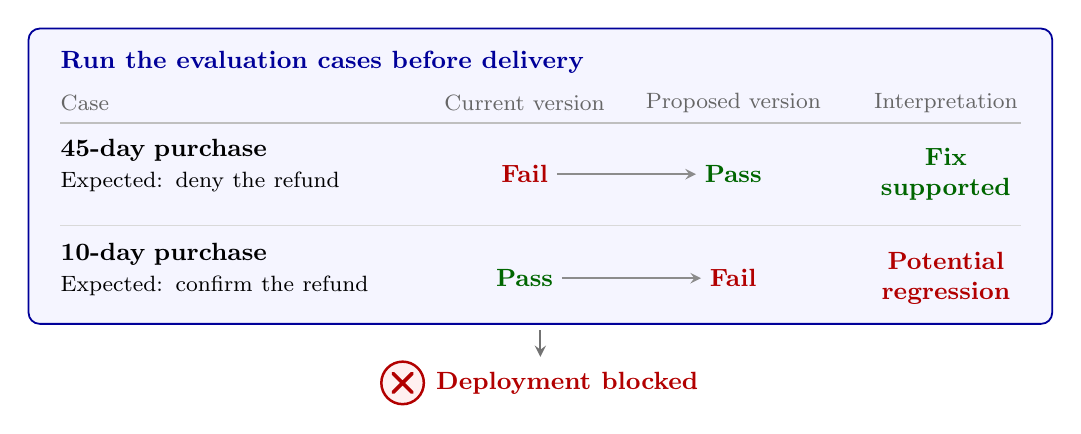
\begin{tikzpicture}[
  panel/.style={rounded corners=4pt, line width=0.65pt},
  heading/.style={anchor=north west, font=\small\bfseries, inner sep=0pt},
  colhead/.style={font=\footnotesize, text=black!60, inner sep=0pt},
  casetext/.style={anchor=north west, font=\small, align=left,
    inner sep=0pt, text width=4.6cm},
  badge/.style={font=\small\bfseries, minimum height=0.5cm, inner sep=3pt},
  pass/.style={badge, text=green!40!black},
  fail/.style={badge, text=red!70!black},
  outcome/.style={font=\small\bfseries, align=center, inner sep=0pt},
  change/.style={->, >=stealth, draw=black!45, line width=0.7pt},
  flow/.style={->, >=stealth, draw=black!55, line width=0.8pt}
]
  % Results of both cases on the current and proposed versions.
  \draw[panel, draw=blue!60!black, fill=blue!4]
    (0,0) rectangle (13,-3.75);
  \node[heading, text=blue!60!black] at (0.4,-0.28)
    {Run the evaluation cases before delivery};

  \node[colhead, anchor=west] at (0.4,-0.95) {Case};
  \node[colhead] at (6.3,-0.95) {Current version};
  \node[colhead] at (8.95,-0.95) {Proposed version};
  \node[colhead] at (11.65,-0.95) {Interpretation};
  \draw[black!25, line width=0.5pt] (0.4,-1.2) -- (12.6,-1.2);

  \node[casetext] at (0.4,-1.4)
    {\textbf{45-day purchase}\\
     {\footnotesize Expected: deny the refund}};
  \node[fail] (c1) at (6.3,-1.85) {Fail};
  \node[pass] (p1) at (8.95,-1.85) {Pass};
  \draw[change] (c1.east) -- (p1.west);
  \node[outcome, text=green!40!black] at (11.65,-1.85) {Fix\\supported};

  \draw[black!15, line width=0.5pt] (0.4,-2.5) -- (12.6,-2.5);

  \node[casetext] at (0.4,-2.72)
    {\textbf{10-day purchase}\\
     {\footnotesize Expected: confirm the refund}};
  \node[pass] (c2) at (6.3,-3.17) {Pass};
  \node[fail] (p2) at (8.95,-3.17) {Fail};
  \draw[change] (c2.east) -- (p2.west);
  \node[outcome, text=red!70!black] at (11.65,-3.17)
    {Potential\\regression};

  \draw[flow] (6.5,-3.83) -- (6.5,-4.17);

  % Delivery decision under the team's policy: a blocked deployment.
  \begin{scope}[shift={(4.75,-4.5)}, draw=red!70!black]
    \draw[fill=red!6, line width=0.9pt] (0,0) circle (0.27);
    \draw[line width=1.3pt, line cap=round]
      (-0.12,-0.12) -- (0.12,0.12) (-0.12,0.12) -- (0.12,-0.12);
  \end{scope}
  \node[anchor=west, font=\small\bfseries, text=red!70!black, inner sep=0pt]
    at (5.17,-4.5) {Deployment blocked};
\end{tikzpicture}
